\documentclass[
	%nofont % Vypnutí přednastaveného fontu Times New Roman
]{cz_sablona}


\title{IPA overview}
\author{Zubař}
\date{\today}

\usepackage{svg}
\usepackage{float} %added so I can place figures [H]
\usepackage{textcomp}
\usepackage{enumitem}
\usepackage{xcolor}

% Make list spacing smaller
\setlist[itemize]{noitemsep, topsep=0.25em, parsep=0pt, partopsep=0pt}
\setlist[enumerate]{noitemsep, topsep=0.25em, parsep=0pt, partopsep=0pt}


\newcommand{\reg}[1]{\texttt{\textcolor{red}{#1}}}
\newcommand{\mem}[1]{\texttt{\textcolor{blue}{#1}}}
\definecolor{darkgreen}{rgb}{0.0, 0.5, 0.0}
\newcommand{\const}[1]{\texttt{\textcolor{darkgreen}{#1}}}
\newcommand{\instr}[1]{\texttt{\textbf{#1}}}

\begin{document}

\maketitle

\thispagestyle{empty}
\newpage
\tableofcontents
\thispagestyle{empty}
\newpage
\section{MMX}
\subsection{Info}
Rozšíření uděláno pro zpracování multimedií.\\
Nepřináší žádný nový hardware, ale parazituje na FPU.\\[0.5em]
\textbf{Osm 64 bitových registrů} (MM0-MM7)\\[0.5em]
Znamená to, že z 80 bitů registru je využíváno pouze 64, zbylých 16 je nevyužitých.
Umí pracovat jenom s celými čísly, but signed nebo unsigned.\\

\noindent
Používá přípony instrukcí, aby určil typ, tedy:
\begin{itemize}
    \item \textit{i128} signed 128 integer
    \item \textit{i64} signed 64 integer
    \item \textit{u64} unsigned 64 integer
    \item \textit{i32} signed 32 integer
    \item \textit{u32} unsigned 32 integer
    \item \textit{i16} signed 16 integer
    \item \textit{u16} unsigned 16 integer
    \item \textit{i8} signed 8 integer
    \item \textit{u8} unsigned 8 integer
\end{itemize}

\noindent
\textbf{Aritmetika MMX}
\begin{itemize}
    \item \textbf{Maskovací}\\
    To co se nevleze po provedení se zahodí.\\
    CF (carry flag) a OF (overflow flag) se ignorují.
    \item \textbf{Znamenková saturace}\\
    Pokud přeteče pozitivně, nastaví se na max, naopak na min.
    \item \textbf{ Beznaménková saturace}\\
    Pokud přeteče pozitivně, nastaví se na max, naopak na min(tedy 0).
\end{itemize}

\subsection{Instrukce MMX (a SSE do budoucna)}
\noindent
\begin{itemize}
    \item \reg{mm} -- reprezentuje registr MMX
    \item \mem{m64} -- reprezentuje 64bitový blok paměti
    \item \mem{m32} -- reprezentuje 32bitový blok paměti
    \item \const{imm8} -- je konstantní 8bitová hodnota
    \item \reg{r32} -- je 32bitový registr pro obecné použití
    \item \reg{r64} -- je 64bitový registr pro obecné použití
    \item \reg{r}/\mem{m32} -- říká, že si můžeme vybrat, zda operand bude 32bitový registr nebo 32bitový blok v paměti
    \item \reg{mm}/\mem{m64} -- nám dává na výběr registr MMX a 64bitový blok paměti
    \item \reg{\textsuperscript{x}mm} -- nám dává na výběr registr MMX nebo XMM(SSE)
\end{itemize}

\subsubsection{Instrukce přesunu}
\noindent
Základní instrukce pro přesun dat mezi registry MMX, obecnými registry a pamětí:

\begin{itemize}
    \item \instr{MOVD} \reg{mm}\textbf{,} \reg{r}/\mem{m32}
    -- přesune 32bitovou hodnotu z 32bitového registru nebo paměti do MMX registru a naopak.
    \item \instr{MOVQ} \reg{\textsuperscript{x}mm}\textbf{,} \mem{m64}/\reg{r64}
    -- přesune 64bitový blok z registru do registru nebo paměti a naopak.
    \item \instr{MOVQ} \reg{\textsuperscript{x}mm}\textbf{,} \reg{r64}
    -- přesune 64bitový blok z registru do registru obecneho použití a naopak.
\end{itemize}

\subsubsection{Instrukce aritmetické}
\instr{PADD(S|U|nic)(B|W|D)} \reg{\textsuperscript{x}mm}\textbf{,} \reg{\textsuperscript{x}mm}/\mem{m64}\\
\instr{PSUB(S|U|nic)(B|W|D)} \reg{\textsuperscript{x}mm}\textbf{,} \reg{\textsuperscript{x}mm}/\mem{m64}

\noindent
Sečte nebo odečte registry nebo registr s pamětí.\\
\texttt{S|U|nic} určí aritmetiku (maskovací, znaménkovou saturaci, beznaménkovou saturaci)\\
\texttt{B|W|D} určí velikost operandu (8, 16, 32 bitů)
\\[0.5em]
\instr{PMUL(L|H)W} \reg{\textsuperscript{x}mm}\textbf{,} \reg{\textsuperscript{x}mm}/\mem{m64}\\
Vynásobí znamenkově 16bitové operandy a uloží buď dolních (L) nebo horních (H) 16 bitů výsledku.
\\[0.5em]
\instr{PMADDWD} \reg{\textsuperscript{x}mm}\textbf{,} \reg{\textsuperscript{x}mm}/\mem{m64}
\textit{Packed Multiply and Add Words into Double}\\
Vynásobí znamenkově 16bitové operandy, sečte levé a pravé tyhle dva 32 bitové výsledky uloží.
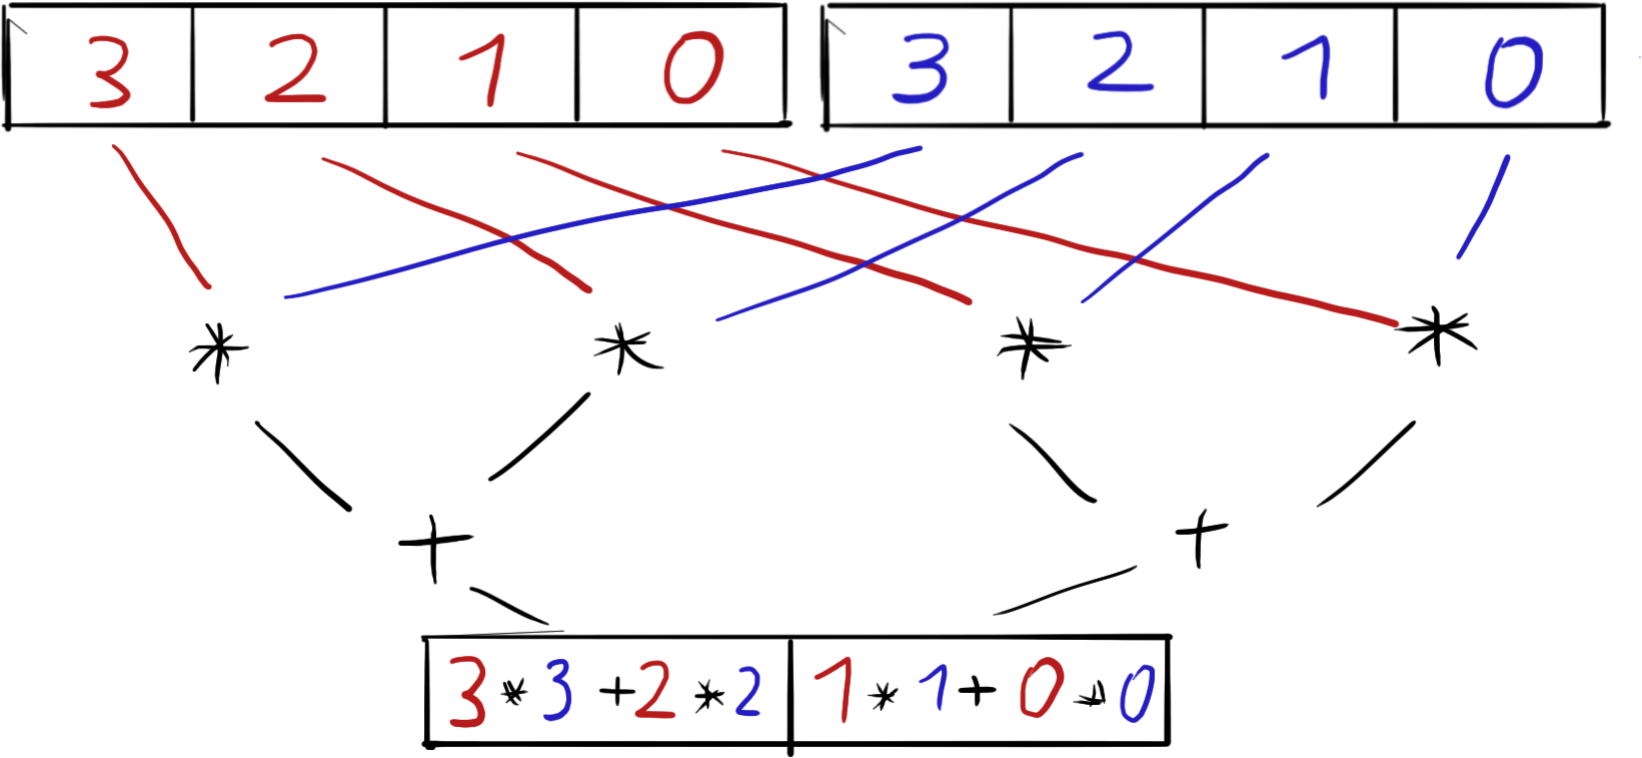
\includegraphics[width=0.5\textwidth]{pics/PMADDWD.png}

\subsubsection{Instrukce porovnání}
\instr{PCMP(EQ|GT)(B|W|D)} \reg{\textsuperscript{x}mm}\textbf{,} \reg{\textsuperscript{x}mm}/\mem{m64}\\
Vytvoří masku porovnáním operandů.
\subsubsection{Instrukce konverzí}
\instr{PACK(SS|US)(WB|DW)} \reg{\textsuperscript{x}mm}\textbf{,} \reg{\textsuperscript{x}mm}/\mem{m64}\\
Zpackuje tedy vezme dva velké typy a nerve je do menších.\\
\textit{SS|US} určí aritmetiku (znaménkovou nebo beznaménkovou saturaci)\\
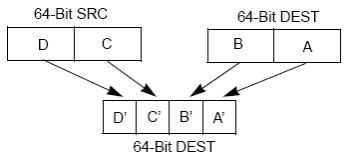
\includegraphics[width=0.5\textwidth]{pics/PACKSS.png}

\subsubsection{Instrukce expanzí}
\instr{PUNPCK(L|H)(B|W|D)} \reg{\textsuperscript{x}mm}\textbf{,} \reg{\textsuperscript{x}mm}/\mem{m64}\\
Vezme horni nebo dolní část obou registrů a proloží je do výsledku.\\
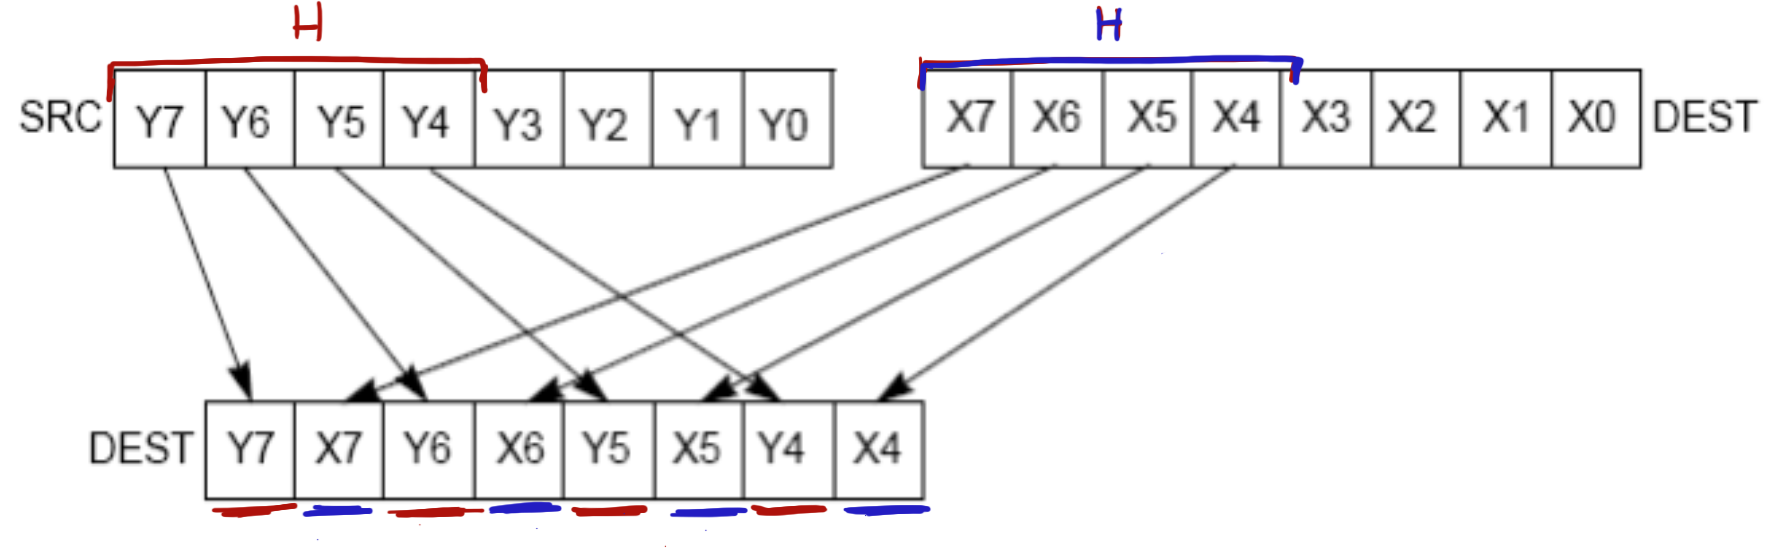
\includegraphics[width=0.8\textwidth]{pics/PUNPCK.png}\\
Jak u Hight i Low verze je je první nejnižší bit vždy z DEST.
\subsubsection{Logické instrukce}
\instr{PAND} \reg{\textsuperscript{x}mm}\textbf{,} \reg{\textsuperscript{x}mm}/\mem{m64}\\
\instr{PANDN} \reg{\textsuperscript{x}mm}\textbf{,} \reg{\textsuperscript{x}mm}/\mem{m64}\\
\instr{POR} \reg{\textsuperscript{x}mm}\textbf{,} \reg{\textsuperscript{x}mm}/\mem{m64}\\
\instr{PXOR} \reg{\textsuperscript{x}mm}\textbf{,} \reg{\textsuperscript{x}mm}/\mem{m64}\\
Prostě udělá to operaci idk.
\\[0.5em]
\instr{EMMS} \textit{Empty MMx State} \\
MUSÍ se zavolat mezi používáním MMX a FPU.\\
Obnoví FPU registry, které MMX používá, takže se můžou použít z FPU.

\subsubsection{Instrukce posunu}
\instr{PS(L|R)L(W|D|Q)} \reg{\textsuperscript{x}mm}\textbf{,} \reg{\textsuperscript{x}mm}/\mem{m64}\\
\instr{PS(L|R)L(W|D|Q)} \reg{\textsuperscript{x}mm}\textbf{,} \const{imm8}\\
Shiftne jednotlivé části(bloky) v registrech doleva nebo doprava logicky, tedy doplni nuly.\\
\texttt{L|R} určí směr posunu (Left, Right)\\
\texttt{W|D|Q} určí velikost operandu (16, 32, 64 bitů)
\\[0.5em]
\instr{PSRA(W|D)} \reg{\textsuperscript{x}mm}\textbf{,} \reg{\textsuperscript{x}mm}/\mem{m64}\\
\instr{PSRA(W|D)} \reg{\textsuperscript{x}mm}\textbf{,} \const{imm8}\\
Arithmetic shift, tedy zachová znaménko (quad verze neexistuje).

\section{SSE a AVX}
\subsection{Info SSE}
\textbf{Osm 128 bitových registrů} (XMM0-XMM7)\\
\textbf{32 bitový kontrolní registr}\\
Tyto registry již jsou reálné fyzické registry, na rozdíl od MMX.\\
SSE taky už umí pracovat s floaty a rozlišuje mezi skalární a vektorovou operací.\\
Skalární operace pracuje jenom s tím úplně nejnižším blokem,
vektorová je to co bylo u MMX.
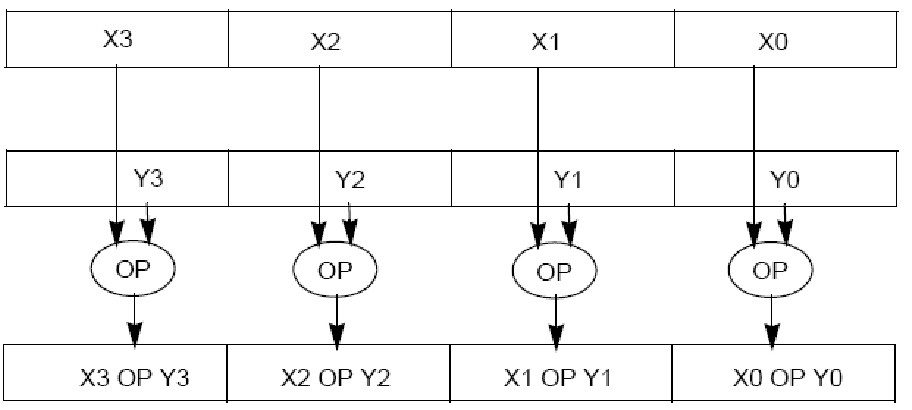
\includegraphics[width=0.5\textwidth]{pics/vektorovaOperace.png}
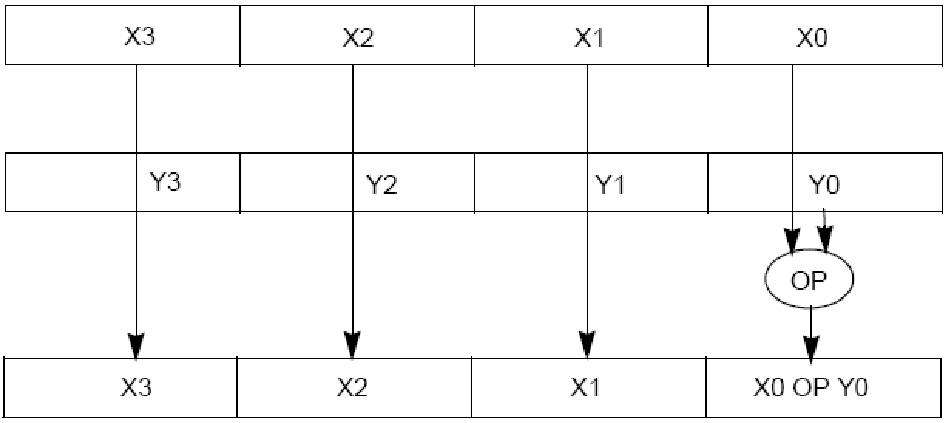
\includegraphics[width=0.5\textwidth]{pics/skalarniOperace.png}
SSE puvodní má \textbf{jenom floaty} celá čísla neumí.\\
SSE2 přidává double a celá čísla, a je tedy plnou nahradou MMX.\\
Z obou verzí tedy pak vzniknou tyhle nové přípony instrukcí:
\begin{itemize}
    \item \textit{SS} -- scalar single (32 bitů, tedy jeden float)
    \item \textit{PS} -- packed single (128 bitů, tedy čtyři floaty)
    \item \textit{SD} (SSE2) -- single double (64 bitů, tedy jeden double)
    \item \textit{PD} (SSE2) -- packed double (128 bitů, tedy dva doubly)
\end{itemize}

\subsection{Info AVX}
AVX je rozšíření SSE.\\
\textbf{Šestnáct 256 bitových registrů} (YMM0-YMM15)\\
Spodnich 128 jsou XMM registry.\\
Všechny instrukce se rozšířují na 256 bitů, vleze se tam toho víc atd.\\
AVX ještě nemá celočíselné instrukce pro 256 bitů, to přidává až AVX2.\\
Zavádí 3 operandové instrukce (dva zdrojové registry a jeden cílový)\\
Tyto instrukce mají předponu \textit{V}, tím se taky odlišují od SSE, jinak
ale vetšina instrukcí z SSE je úplně stejně v AVX.\\
AVX2 taky přidává různé quality of life instrukce.

\subsection{Řídící registr MXCSR}
\begin{itemize}
    \item \textbf{Vyjímky} -- bity které jsou nastaveny pokud proběhla nějaká vyjímka
    \item \textbf{DNZ} -- Denormals Are Zeros -- 1 $\rightarrow$ denormalní čísla jsou nula\\
    denormalní čísla jsou tak malá, že nejde normalizovat mantisa
    \item \textbf{Maskování vyjímek} maskuje vyjímky\\
    místo crashnutí jen ji jen nastaví\\
    a pak tam dá tu nejvíc smyslnou hodnotu (nekonečno, NaN, ...)
    \item \textbf{RC} -- Rounding Control -- určuje jak se zaokrouhluje\\
    00 -- round to nearest\\
    01 -- round down\\
    10 -- round up\\
    11 -- floor
    \item \textbf{Flush to zero} -- 1 $\rightarrow$ při podtečení je výsledek nula
\end{itemize}

\subsection{Instrukce SSE (a AVX)}
\begin{itemize}
    \item \reg{*mm} -- reprezentuje registr SSE nebo AVX (xmm/ymm)
    \item \reg{xmm} -- reprezentuje registr SSE (xmm)
    \item \reg{ymm} -- reprezentuje registr AVX (ymm)
    \item \mem{m*} -- block pamětí podle velikosti operace
\end{itemize}
Někde nenapíšu AVX verzi explicitně, což by mělo znamenat, že funguje úplně stejně
jako SSE, jenom se to zapíše do dst a ty dva src se nezmění.

\subsubsection{Instrukce přesunu}
\instr{[V]MOV(A|U)P(S|D)} \reg{*mm}\textbf{,} \reg{*mm}/\mem{m*}\\
\instr{[V]MOV(A|U)P(S|D)} \reg{*mm}/\mem{m*}\textbf{,} \reg{*mm}\\
Přesune data mezi registry nebo registrem a pamětí.\\
\texttt{A|U} určí zda se jedná o aligned nebo unaligned\\
Aligned znamená, že pokud adresa není zarovnána na velikost čtené hodnoty, dojde k chybě.\\
\texttt{S|D} určí zda se jedná o float nebo double
\\[0.5em]
\instr{VLDQU} \reg{*mm}\textbf{,} \mem{m*}\\
Vlastně to co MOVU
\\[0.5em]
\instr{[V]MOVS(S|D)} \reg{xmm}\textbf{,} \reg{xmm}/\mem{m*}\\
Skalární move, pracuje jen s nejnižším blokem (32 nebo 64 bitů), vynuluje zbytek.
\\[0.5em]
\instr{VMOVS(S|D)} \reg{xmm}\textbf{,} \reg{xmm}\textbf{,} \reg{xmm}\\
Vezme src1 a src2 a přesně v tomto položení je uloží do dst.\\
pro S: \texttt{d[127:32] = s1[127:32], d[31:0] = s2[31:0]}\\
pro D: \texttt{d[127:64] = s1[127:64], d[63:0] = s2[63:0]}
\\[0.5em]
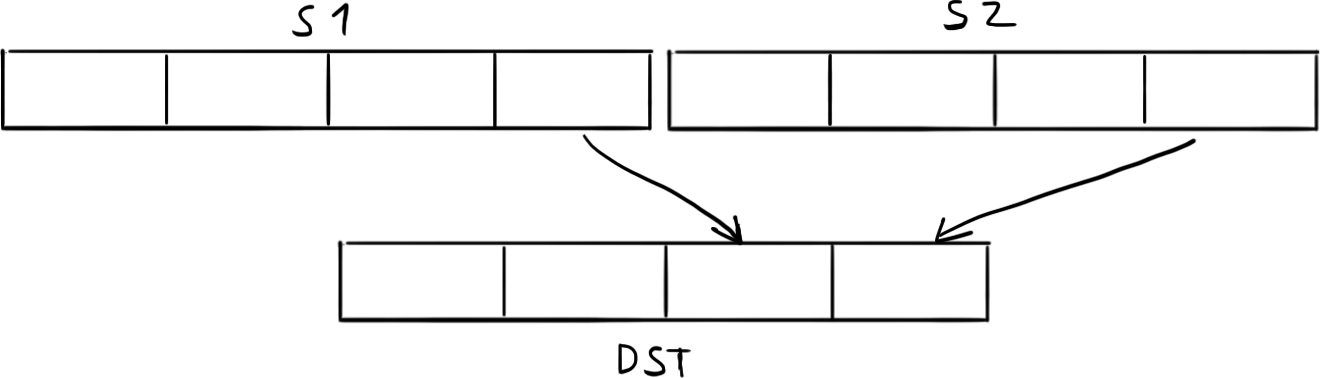
\includegraphics[width=0.8\textwidth]{pics/VMOVSS.png}
\\[0.5em]
\instr{MOVPLP(S|D)} \reg{xmm}\textbf{,} \reg{xmm}/\mem{m*}\\
\instr{MOVPLP(S|D)} \reg{xmm}/\mem{m*}\textbf{,} \reg{xmm}\\
Moves the lower 64 bits, does not zero the upper bits.
\\[0.5em]
\instr{VMOVLP(S|D)} \reg{xmm}\textbf{,} \reg{xmm}\textbf{,} \mem{m64}\\
Functions like VMOVS(S|D) but with memory and without zeroing upper bits.\\
When writing into memory, it only has two operands, and functions as expected.
\\[0.5em]
\instr{MOVHP(S|D)} \reg{xmm}\textbf{,} \reg{xmm}/\mem{m*}\\
\instr{MOVHP(S|D)} \reg{xmm}/\mem{m*}\textbf{,} \reg{xmm}\\
\instr{VMOVHP(S|D)} \reg{xmm}\textbf{,} \reg{xmm}\textbf{,} \mem{m64}\\
Similar to the Lower moves, but operates on the upper 64 bits of the XMM register.
\\[0.5em]
\instr{MOV(LH|HL)PS} \reg{xmm}\textbf{,} \reg{xmm}\\
Přesune dolní polovinu jednoho registru do horní poloviny druhého a naopak.\\
\instr{VMOV(LH|HL)PS} \reg{xmm}\textbf{,} \reg{xmm}\textbf{,} \reg{xmm}\\
LH $\leftarrow$ dH = s2L, dL = s1L\\
HL $\leftarrow$ dH = s1H, dL = s2H
\\[0.5em]
\instr{[V]MOVMSKP(S|D)} \reg{r32/64}\textbf{,} \reg{*mm} 
\textit{(Move Masked Scalar Packed Single/Double)} \\
Zkopíruje jenom nevyšší bit každého bloku do obecného registru.
\\[0.5em]
\instr{[V]MOV(S|D)(H|L)DUP} \reg{*mm}\textbf{,} \reg{*mm}/\mem{m*}\\
Vezme každý druhý single nebo double zleva nebo zprava zkopíruje ho do
dst a pak je naduplikuje jednou tím stejným směrem.\\
Obrazky jsou zleva verze high a verze low.\\
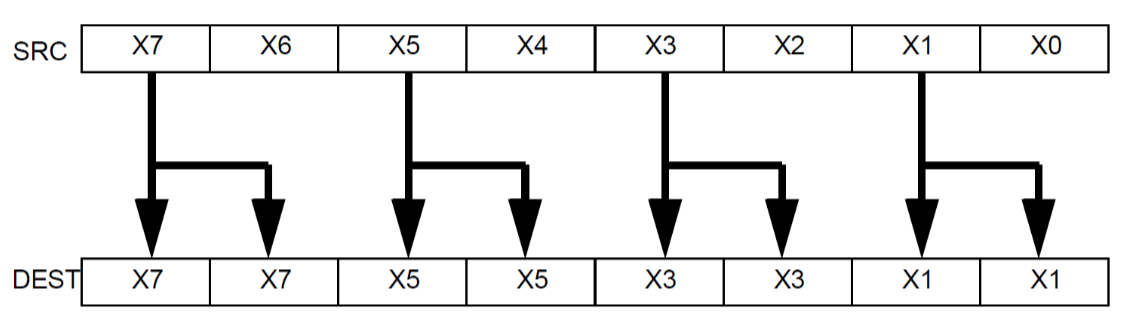
\includegraphics[width=0.5\textwidth]{pics/MOVSHDUP.png}
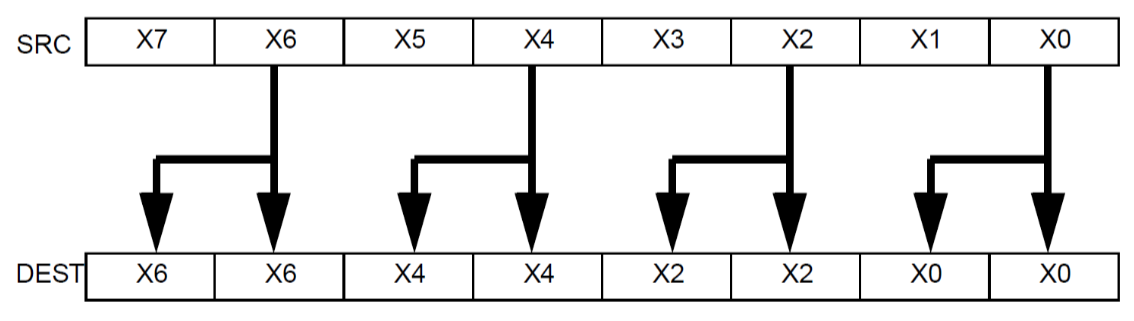
\includegraphics[width=0.5\textwidth]{pics/MOVSLDUP.png}

\subsubsection{Záměny složek}
\instr{SHUFP(S|D)} \reg{xmm}\textbf{,} \reg{xmm}/\mem{m128}\textbf{,} \const{imm8}\\
\instr{VSHUFP(S|D)} \reg{*mm}\textbf{,} \reg{*mm}\textbf{,} \reg{*mm}/\mem{m*}\textbf{,} \const{imm8}\\
Podle pozic definovanými dvoj bity v \const{imm8} přehází věci ze src do dest.\\
\texttt{V} verze udělá se src1 to stejný a src2 přehází stejným způsobem
ale do horní poloviny dst když se to tam vleze.\\
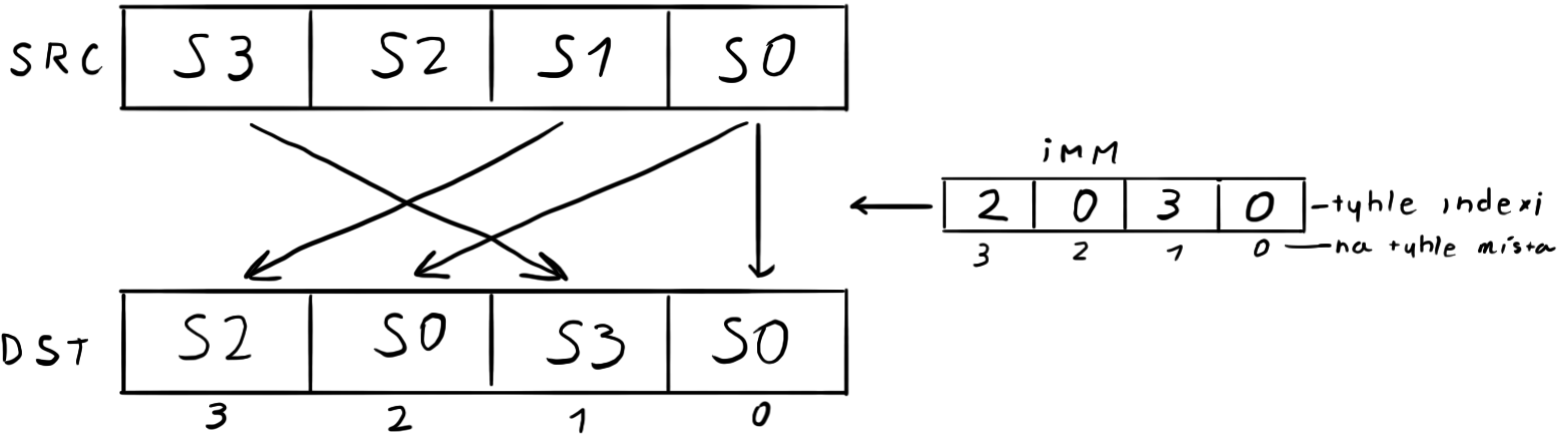
\includegraphics[width=0.8\textwidth]{pics/SHUFP.png}

\subsubsection{Extrakce složek vektorů}
\instr{UNPCK(H|L)P(S|D)} \reg{xmm}\textbf{,} \reg{xmm}/\mem{m*}\\
\instr{VUNPCK(H|L)P(S|D)} \reg{*mm}\textbf{,} \reg{*mm}\textbf{,} \reg{*mm}/\mem{m*}\\
Vezme horní nebo dolní částí obou registrů a promíchá je do výsledku.\\
Nejnižší bit je vždy z DEST nebo SRC1 pokud je V verze.\\
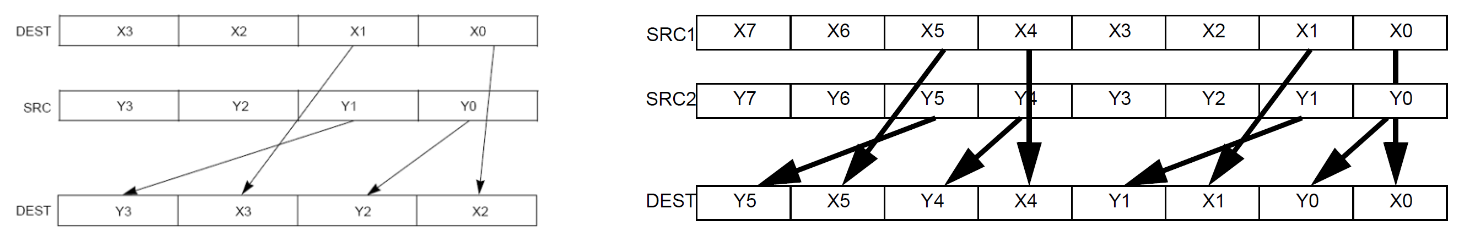
\includegraphics[width=1\textwidth]{pics/UNPCK.png}

\subsubsection{Porovnání}
\instr{CMP(SS|PS|SD|PD)} \reg{xmm}\textbf{,} \reg{xmm}/\mem{m128}\textbf{,} \const{imm8}\\
\instr{VCMP(SS|PS|SD|PD)} \reg{*mm}\textbf{,} \reg{*mm}\textbf{,} \reg{*mm}/\mem{m*}\textbf{,} \const{imm8}\\
Vygeneruje masku porovnáním operandů.\\
Porovnání dáno \const{imm8}, ale lze i pseudoinstrukcemi (e.g. \instr{CPMLEPS})
\\[0.5em]
\instr{[V][U]COMIS(S|D)} \reg{xmm}\textbf{,} \reg{xmm}/\mem{m*}\\
Porovná skalární floaty nebo doubly a nastaví CF, PF, ZF podle výsledku.\\
\texttt{U} Necrashne pokud jsou čísla neporovnatelná.

\subsection{Aritmetické instrukce SSE a AVX}
Tady je jsou všechny klasické aritmetické instrukce, ale pro floaty a doubly.\\
Aplikují se nad sebou dle typu, případně jenom nad nejnižším blokem když je to SS/SD.\\
Při AVX instrukcích je třetí operand buď registr nebo paměť, zbytek jsou registry.
\\[0.5em]
\instr{[V]ADDSUBP(S|D)} \reg{*mm}\textbf{,} \reg{*mm}/\mem{m*}\\
Sečte liché složky a odečte sudé.\\
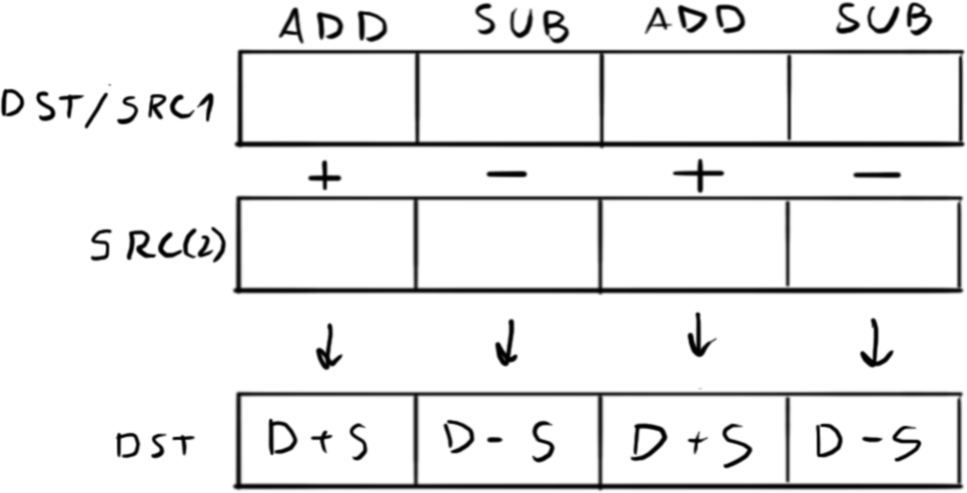
\includegraphics[width=0.5\textwidth]{pics/ADDSUB.png}
\\[0.5em]
\instr{[V]H(ADD|SUB)P(S|D)} \reg{*mm}\textbf{,} \reg{*mm}/\mem{m*}\\
Sečte/odečte sousední složky\\
H $\rightarrow$ horizontal, pracuje s složkami ve stejném registru.\\
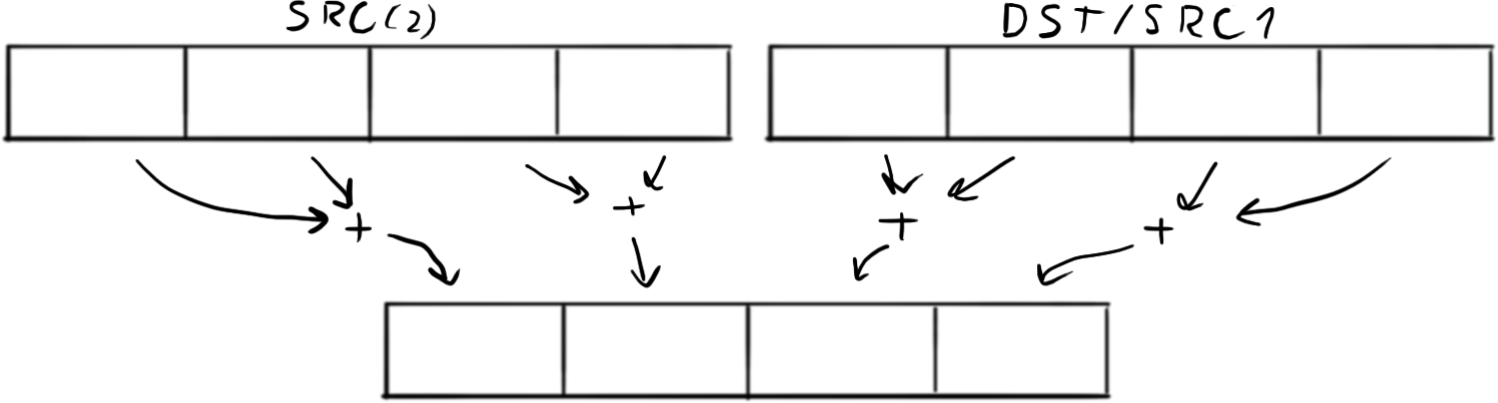
\includegraphics[width=0.8\textwidth]{pics/HADD.png}

\subsubsection{Konverze}
Instrukce má formát \instr{[V]CVT[T](S|P)(S|D|I)2(S|P)(S|D|I)}. případně DQ typ\\
\texttt{T} určuje truncation, takže jestli ořezává při konverzi.\\
Potom převede jednu věc na druhou.\\
Pokud je packed, tak je to mezi registry SSE nebo pamětí.\\
Pokud je scalar, tak je to mezi SSE registrem a pamětí nebo registrem obecného použití.\\
\texttt{S|D|I} určuje typy, tedy single, double nebo integer.\\
\texttt{S|P} určuje jestli je to skalární nebo vektorová operace.\\
\texttt{DQ} V tomto případě jsou to dvojslova (32-bit) celočíselná.\\
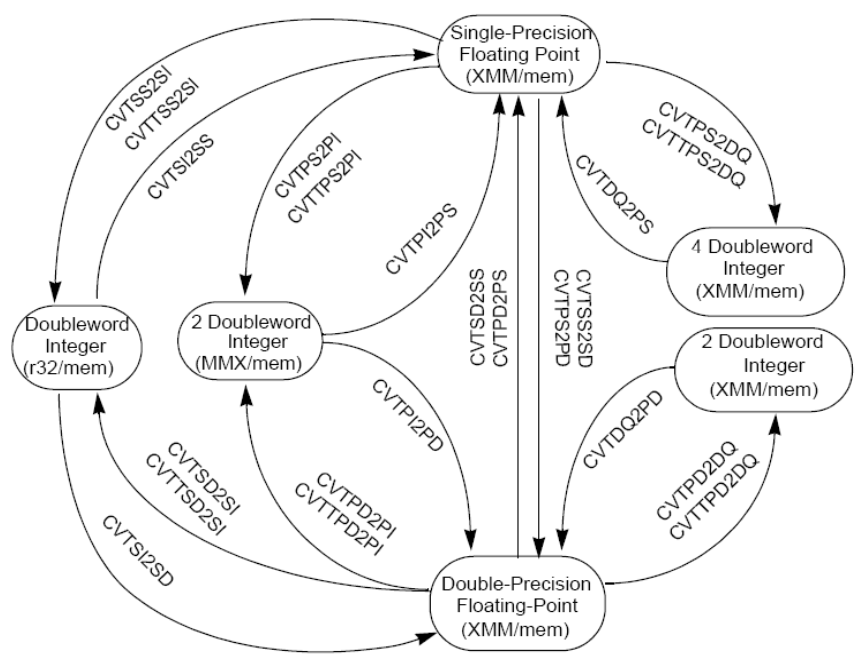
\includegraphics[width=0.8\textwidth]{pics/conversions.png}

\subsubsection{Celočíselné instrukce}
\instr{[V]PAVG(B|W)} \reg{*mm}\textbf{,} \reg{*mm}/\mem{m*}\\
Dělá průměr dvou operandů vektorově.
\\[0.5em]
\instr{[V]PEXTRW} \reg{r32/64}/\mem{m16}\textbf{,} \reg{*mm}\textbf{,} \const{imm8}\\
Vyextrahuje hodnotu z src na indexu daném \const{imm8} a uloží dolů do obecného registru nebo paměti.
\\[0.5em]
\instr{[V]INSERTW} \reg{*mm}\textbf{,} \reg{r32/64}/\mem{m16}\textbf{,} \const{imm8}\\
Vloží hodnotu z dolní části obecného registru nebo paměti do src na index daný \const{imm8}.
\\[0.5em]
\instr{[V]P(MIN|MAX)(U|S)(B|W)} \reg{*mm}\textbf{,} \reg{*mm}/\mem{m*}\\
Určí minimální nebo maximální hodnotu mezi dvěma operandy vektorově.
\\[0.5em]
\instr{[V]PMOVMSKB} \reg{r32/64}\textbf{,} \reg{*mm}\\
Zkopíruje nejvyšší bit z každých osm bitů do jedněch osmi bitů do obecného registru.
\\[0.5em]
\instr{[V]PMULHUW} \reg{*mm}\textbf{,} \reg{*mm}/\mem{m*}
\textit{Packed Multiply Higher Unsigned Words}\\
Vynásobí wordy a uloží z vysledku horni části do dst.\\
\\[0.5em]
\instr{[V]PSADBW} \reg{*mm}\textbf{,} \reg{*mm}/\mem{m*}
\textit{Packed Sum of Absolute Differences of Bytes into Word}\\
Udělá absolutní rozdíly všech byte a pak se sečte do spodního wordu dst.
\\[0.5em]
\instr{[V]PMULUDQ} \reg{*mm}\textbf{,} \reg{*mm}/\mem{m*}\\
Vynásobí unsigned doubly a uloží je to quadword do dst.\\
\instr{[V]PS(L|R)LDQ} \reg{*mm}\textbf{,} \reg{*mm}/\mem{m*}\textbf{,} \const{imm8}\\
Posune obsah double quad wordů logicky, což pro xmm je cely registr.
\\[0.5em]
\textbf{Nové přesuny}
\\[0.5em]
\instr{MOVDQA} \reg{xmm}\textbf{,} \reg{xmm}/\mem{m128}\\
Přesune dvě čtyřslova mezi pamětí a XMM registrem nebo mezi dvěma XMM registry.\\
Paměť musí být zarovnaná na 16bytovou hranici.\\[0.5em]
\instr{MOVDQU} \reg{xmm}\textbf{,} \reg{xmm}/\mem{m128}\\
Stejná jako MOVDQA, ale paměť nemusí být zarovnaná.\\[0.5em]
\instr{MOVQ2DQ} \reg{xmm}\textbf{,} \reg{mm}\\
Přesune čtyřslové celé číslo z MMX do dolní části XMM registru a zbytek vynuluje.\\[0.5em]
\instr{MOVDQ2Q} \reg{mm}\textbf{,} \reg{xmm}\\
Přesune dolní čtyřslovo z XMM registru do MMX registru.\\[0.5em]
\instr{PSHUFLW} \reg{xmm}\textbf{,} \reg{xmm}/\mem{m128}\textbf{,} \const{imm8}\\
Přehází slova v dolním čtyřslovu zdrojového operandu podle pořadí daného 8bitovou konstantou.\\[0.5em]
\instr{PSHUFHW} \reg{xmm}\textbf{,} \reg{xmm}/\mem{m128}\textbf{,} \const{imm8}\\
Přehází slova v horním čtyřslovu zdrojového operandu podle pořadí daného 8bitovou konstantou.\\[0.5em]
\instr{PSHUFD} \reg{xmm}\textbf{,} \reg{xmm}/\mem{m128}\textbf{,} \const{imm8}\\
Přehází dvojslova ve zdrojovém operandu podle pořadí definovaného 8bitovou konstantou.\\[0.5em]
\instr{PUNPCKHQDQ} \reg{xmm}\textbf{,} \reg{xmm}/\mem{m128}\\
Proloží horní čtyřslovo zdroje s horním čtyřslovem cíle a výsledek uloží do cíle.\\[0.5em]
\instr{PUNPCKLQDQ} \reg{xmm}\textbf{,} \reg{xmm}/\mem{m128}\\
Proloží dolní čtyřslovo zdroje s dolním čtyřslovem cíle a výsledek uloží do cíle.

\subsection{SSSE3 instrukce}
\instr{[V]PSIGN(B|W|D)} \reg{*mm}\textbf{,} \reg{*mm}/\mem{m*}\\
Jakoby vezme znaménka z src a vynasobí jimi dst.\\
Pokud je v src nula, da nulu i do dst.
\\[0.5em]
\instr{[V]PABS(B|W|D)} \reg{*mm}\textbf{,} \reg{*mm}/\mem{m*}\\
Udělá absolutní hodnotu všech prvků ve vektoru.
\\[0.5em]
\instr{[V]H(ADD|SUB)[S](W|D)} \reg{*mm}\textbf{,} \reg{*mm}/\mem{m*}\\
Zase horizontalni instrukce, tedy sčitaj/odčitaj sousedy.\\
\texttt{S} znamená, že se použije saturace.
\\[0.5em]
\instr{[V]PALIGNR} \reg{*mm}\textbf{,} \reg{*mm}/\mem{m*}\textbf{,} \const{imm8}\\
Vezme dst a src (případně src2), zkonkatenuje je, šoupne doprava
dle \const{imm8} a výsledek uloží do dst.\\
\instr{[V]SHUFB} \reg{*mm}\textbf{,} \reg{*mm}/\mem{m*}\\
Přehází dst (nebo src1) dle obsahu src (nebo src2).\\
Každý byte určuje jaký bajt z dst (nebo src1) se má dostat do výsledku.\\
Negativní hodnota znamená, že se do výsledku dostane nula.
\\[0.5em]
\instr{[V]PMULHRW} \reg{*mm}\textbf{,} \reg{*mm}/\mem{m*}\\
\textit{Packed Multiply High Round and Scale for Words}\\
Vynásobí wordy, přičemž výsledek se zaokrouhlí a pak se uloží horní část výsledku do dst.
\\[0.5em]
\instr{[V]MADDUBSW} \reg{*mm}\textbf{,} \reg{*mm}/\mem{m*}\\
\textit{Multiply and Add Unsigned and Signed Bytes to Signed Words}\\
Vezme byty z dst a src, dst signed, src unsigned, \\
vynásobí je, sečte sousední a nakonec zapíše do dst jako signed word.

\subsection{SSE4 instrukce}
\instr{[V]MOV(SX|ZX)(B|W|D|Q)(B|W|D|Q)} \reg{*mm}\textbf{,} \reg{*mm}/\mem{m*}\\
Kopíruje data mezi registry s tím, že je při kopírování rozšiřuje
(tzn musi byt z mensiho na vetsi typ).\\
\texttt{SX|ZX} určuje jestli je to signed nebo unsigned extension.\\
Jinak je to toho prvniho typu na druhy prostě.
\\[0.5em]
\instr{[V]PACKUSDW} \reg{*mm}\textbf{,} \reg{*mm}/\mem{m*}
\textit{Pack Unsigned with Saturation from DWords to Words}\\
Zpackuje dvojslova z dst i src do unsigned wordů v dst.
\\[0.5em]
\instr{[V]DPP(S|D)} \reg{*mm}\textbf{,} \reg{*mm}/\mem{m*}\textbf{,} \const{imm8}\\
\textit{Dot Product of Packed Single/Double}\\
Děká maskovaný skalarni součin mezi dvěma vektory.\\
Nejdřív se normálně pronásobí složky, pak se sečtou ty,
které mají v horní části \const{imm8} nastavený bit.\\
Výsledek se pak uloží tam, kde je v dolní části \const{imm8} 
nastavený bit.
\\[0.5em]
\instr{[V]MPSADBW} \reg{*mm}\textbf{,} \reg{*mm}/\mem{m*}\textbf{,} \const{imm8}\\
\textit{Masked Packed Sum of Absolute Differences of Bytes into Words}\\
Použije masku k tomu aby urči kde začnu s počítáním sum absolutních rozdílů.
imm[2] $\times$ 4 je začátek v dst\\
imm[1:0] $\times$ 4 je začátek v src\\
V těch indexech jsou okna o velikosti 4 byte,
s nimi se provede SAD a výsledek se uloží do dst.\\
Pak se posune okno v dst do prava o jeden byte a znovu,
vysledek se uloží do další pozice.\\
Takhle celý osmkrát a je to.
\\[0.5em]
\instr{[V]ROUND(S|P)(S|D)} \reg{*mm}\textbf{,} \reg{*mm}/\mem{m*}\textbf{,} \const{imm8}\\
Zaokrouhlí floaty dle typu na celá signed čísla.\\
Použije \const{imm8} k určení způsobu zaokrouhlování,
stejný jako v RC bitu MXCSR.
\instr{[V]BLEND(PS|PD)} \reg{*mm}\textbf{,} \reg{*mm}/\mem{m*}\textbf{,} \const{imm8}\\
\instr{[V]PBLENDW} \reg{*mm}\textbf{,} \reg{*mm}/\mem{m*}\textbf{,} \const{imm8}\\
V dst nahradí jen ty složky, co mají v \const{imm8} nastavený bit.\\
\instr{[V]BLENDV(PS|PD)} \reg{*mm}\textbf{,} \reg{*mm}/\mem{m*}\textbf{,} \reg{*mm}\\
\instr{[V]PBLENDVB} \reg{*mm}\textbf{,} \reg{*mm}/\mem{m*}\textbf{,} \reg{*mm}\\
Stejné jako předchozí blend, ale místo \const{imm8} se použije maska v registru.
Což jsou vždy nejvyšší bity.
\\[0.5em]
\instr{[V]PMULDQ} \reg{*mm}\textbf{,} \reg{*mm}/\mem{m*}\\
Vynásobí dvojslova jako signed a uloží quadslovo do dst.
\\[0.5em]
\instr{[V]PMULLD} \reg{*mm}\textbf{,} \reg{*mm}/\mem{m*}\\
Vynásobí dvojslova jako signed a uloží spodní část jako dvojslovo do dst.\\
\instr{[V]PCMPEQQ} \reg{*mm}\textbf{,} \reg{*mm}/\mem{m*}\\
Porovná dvojslova jako signed a vytvoří masku.
\\[0.5em]
\instr{[V]EXTRACTPS} \reg{r32}/\mem{m32}\textbf{,} \reg{*mm}\textbf{,} \const{imm8}\\
Vyextrahuje float z src na indexu daném \const{imm8}
a uloží ho do obecného registru nebo paměti.\\
\instr{[V]PEXTR(B|D|Q)} \reg{r32/64}/\mem{m16/32/64}\textbf{,} \reg{*mm}\textbf{,} \const{imm8}\\
Vyextrahuje hodnotu z src na indexu daném \const{imm8}
a uloží ji do obecného registru nebo paměti.\\
\instr{[V]INSERTPS} \reg{*mm}\textbf{,} \reg{r32}/\mem{m32}\textbf{,} \const{imm8}\\
Vloží float z obecného registru nebo paměti do src na index daný \const{imm8}.\\
\instr{[V]PINSR(B|D|Q)} \reg{*mm}\textbf{,} \reg{r32/64}/\mem{m16/32/64}\textbf{,} \const{imm8}\\
Vloží hodnotu z obecného registru nebo paměti do src na index daný \const{imm8}.
\\[0.5em]
\instr{[V]P(MIN|MAX)(S|U)(B|W|D)} \reg{*mm}\textbf{,} \reg{*mm}/\mem{m*}\\
Prostě min max vektorově.\\
\instr{PHMINPOSUW} \reg{*mm}\textbf{,} \reg{*mm}/\mem{m128}
\textit{Packed Horizontal MINimum POSition of Unsigned Words}\\
Vytáhne tun nejmenší prvek ze src, to dá naspod a těsně nad ni dá její index.
\\[0.5em]
\instr{[V]PTEST} \reg{*mm}\textbf{,} \reg{*mm}/\mem{m*}\\
Výjhde li logický AND nula, nastaví ZF.
\\[0.5em]
\instr{MOVNTDQA} \reg{xmm}\textbf{,} \mem{m128}\\
Jako mov, ale umožní procesoru uložit to pomocí burst write,
takže je to jenom optimalizační.
\instr{[V]PCMPGTQ} \reg{*mm}\textbf{,} \reg{*mm}/\mem{m*}\\
Porovnává čtyřslova a tvoří masku.
\\[0.5em]
\instr{[V]PCMP(E|I)STR(I|M)} \reg{xmm}\textbf{,} \reg{xmm}/\mem{m128}\textbf{,} \const{imm8}\\
\textit{Packed CoMPare Explicit/Implicit length STRings and get Index/Masks}\\
\begin{itemize}
    \item E -- explicit length, déllka řetězců jedna a dva je v EAX a EDX
    \item I -- implicit length, řetezec ukončen nulou
    \item M -- mask, v dst bude 16(8) bitová maska
    \item I -- index, v dst bude index prvního (případně posledního) rozdílného znaku
\end{itemize}
Konstanta nám pak udává spoustu dalších možností.\\
\begin{itemize}
    \item \const{imm8[0]} -- se znaménkem nebo bez
    \item \const{imm8[1]} -- 0 $\rightarrow$ byte, 1 $\rightarrow$ word
    \item \const{imm8[3:2]} -- jaký druh porovnání
        \begin{itemize} 
            \item[00] -- equal any (podmnožina)
            \item[01] -- ranges (je někde mezi znaky, vždy po dvojicích)
            \item[10] -- equal each (exact match)
            \item[11] -- equal ordered (podřetězec)
        \end{itemize}
    \item \const{imm8[5:4]} -- změnit výsledek booleanovksou operací
        \begin{itemize}
            \item[00/01] -- nechám stejné
            \item[10] -- invertuju
            \item[11] -- Invertuju pokud je to validní index v src stringu
        \end{itemize}
    \item \const{imm8[6]} -- jak bude výsledek reprezentován\\
        pro masku (M)
        \begin{itemize}
            \item[0] -- nulou rozšířených 16(8) bitů
            \item[1] -- Rozkopíruje je to tu masku do všech prvků dst
        \end{itemize}
        pro index (I)
        \begin{itemize}
            \item[0] -- první rozdílný znak
            \item[1] -- poslední rozdílný znak
        \end{itemize}
\end{itemize}

\noindent
\begin{minipage}[t]{0.48\textwidth}
\centering
\textbf{Nastavení příznaků E}

\vspace{0.5em}
\begin{tabular}{|l|l|}
\hline
CF & $(\mathrm{FinalMask} == 0)?\ 0 : 1$ \\
\hline
ZF & $\mathrm{abs}(\mathrm{EDX}) < 16\ (8)$ \\
\hline
SF & $\mathrm{abs}(\mathrm{EAX}) < 16\ (8)$ \\
\hline
OF & $\mathrm{FinalMask}[0]$ \\
\hline
AF & 0 \\
\hline
PF & 0 \\
\hline
\end{tabular}
\end{minipage}
\hfill
\begin{minipage}[t]{0.48\textwidth}
\centering
\textbf{Nastavení příznaků I}

\vspace{0.5em}
\begin{tabular}{|l|l|}
\hline
CF & $(\mathrm{FinalMask} == 0)?\ 0 : 1$ \\
\hline
ZF & nalezen konec s \\
\hline
SF & nalezen konec d \\
\hline
OF & $\mathrm{FinalMask}[0]$ \\
\hline
AF & 0 \\
\hline
PF & 0 \\
\hline
\end{tabular}
\end{minipage}


\subsection{AVX instrukce}
\instr{VCMP} \reg{*mm}\textbf{,} \reg{*mm}\textbf{,} \reg{*mm}/\mem{m*}\textbf{,} \const{imm8}\\
Od normálního CMP má navíc další options v \const{imm8}\\
Ordered/Unordered -- NaN $\rightarrow$ false/true\\
Quiet/Signaling -- NaN $\rightarrow$ nic/exception
\\[0.5em]
\instr{VZERO(ALL|UPPER)}\\
Vynuluje všechny ymm registry nebo jenom jejich horní polovinu.
\\[0.5em]
\instr{VEXTRACT(F|I)128} \reg{*mm}\textbf{,} \reg{*mm}\textbf{,} \const{imm8}\\
Jak normální extrakce, ale cílem je vekt registr a operuje se s 128 bity.\\
\instr{VINSERT(F|I)128} \reg{*mm}\textbf{,} \reg{*mm}\textbf{,} \reg{*mm}\textbf{,} \const{imm8}\\
Jako insert, vyberu 128 bitů z src2 dle \const{imm8} zbytek doplním z src1 a dám do dst.
\\[0.5em]
\instr{VBROADCAST(SS|SD|F128|I128)} \reg{*mm}\textbf{,} \reg{*mm}/\mem{m*}\\
\instr{VPBROADCAST(B|W|D|Q)} \reg{*mm}\textbf{,} \reg{*mm}/\mem{m*}\\
Rozkopíruje spodní element do zbytku dst.\\
\instr{VMASKMOV(PS|PD)} \reg{*mm}\textbf{,} \reg{*mm}\textbf{,} \mem{m*}\\
\instr{VMASKMOV(PS|PD)} \mem{m*}\textbf{,} \reg{*mm}\textbf{,} \reg{*mm}\\
\instr{VPMASKMOV(D|Q)} \reg{*mm}\textbf{,} \reg{*mm}\textbf{,} \mem{m*}\\
\instr{VPMASKMOV(D|Q)} \mem{m*}\textbf{,} \reg{*mm}\textbf{,} \reg{*mm}\\
Zapisuje na základě masky, dané opět nejvyššími bity src1.
\\[0.5em]
\instr{VPPS(R|L)(L|A)V(D|Q)} \reg{*mm}\textbf{,} \reg{*mm}\textbf{,} \reg{*mm}/\mem{m*}\\
Posune každou složky v src1 o to co je v src2 a dá to do dst.\\
\texttt{R|L} určuje směr posunu, tedy jestli se posouvá vpravo nebo vlevo.\\
\texttt{L|A} určuje jestli se posouvá logicky nebo aritmeticky.
\\[0.5em]
\instr{VPERM[IL](PS|PD)} \reg{*mm}\textbf{,} \reg{*mm}\textbf{,} \reg{*mm}/\mem{m*}\textbf{,} \const{imm8}/\reg{*mm}\\
Promíchá src1 podle \const{imm8} nebo src2 a uloží do dst.\\
\texttt{IL} -- in-line -- Udělá to zvlášt pro horní a spodní polovinu.\\
\instr{VPERM2F128} \reg{*mm}\textbf{,} \reg{*mm}\textbf{,} \reg{*mm}/\mem{m*}\textbf{,} \const{imm8}\\
Promíchá src1 a src2 podle \const{imm8} a uloží do dst.\\
Umí i vynulovat dle \const{imm8}.
\\[0.5em]
\instr{V[P]GATHERxxxx} d, [base+a*scale+disp], b\\
Umí načíst různé rozházené položky z paměti do vektoru.\\
V \texttt{a} jsou indexy, který se ponásobí a šoupnou aby vznikla adresa.\\
V \texttt{b} je maska, která určí, jestli se to načte nebo ne.
Pokud ne, tak se zachová původní hodnota.\\
\texttt{xxxx} určuje typ indexů a co se načítá, což je samo ovlivněno jestli
je to celočíselné nebo ne.
Takže třeba \texttt{VPGATHERDD} má v \texttt{a} indexy jako dvojslova
a načítá data ve dvojslovech,
\texttt{VGATHERQPD} má v \texttt{a} indexy jako quadslova
a načítá data jako double.
\\[0.5em]
\instr{VFMADD(132|231)(PS|PD|SS|SD)} \reg{*mm}\textbf{,} \reg{*mm}\textbf{,} \reg{*mm}
\textit{Fused Multiply-Add}\\
Vynásobí dva operandy a pak přičte třetí,\\
Pořadí dáno čísly, takže třeba 132 znamená (dst $\times$ src2) + src1.\\

\section{ARM}
\subsection{Režimy procesoru}
Zhruba dle snižující se priority:
\begin{itemize}
    \item Přerušení -- obsluha chyby s pamětí
    \item IFQ (Fast Interrupt Request) --
    přerušení s vysokou prioritou
    \item IRQ (Interrupt Request) --
    běžné přerušení
    \item Nedefinovaný -- 
    obsluda použití neznámých instrukcí
    \item Dohližitelský (Supervisor) --
    po reset a SW přerušení
    \item Uživatelský (User) --
    běžné aplikace, neprivilagovaný režim
\end{itemize}
64bit zavádí exception levels.\\
Ty jsou čtyři:
\begin{itemize}
    \item EL0 -- uživatelský režim
    \item EL1 -- kernel
    \item EL2 -- hypervisor
    \item EL3 -- secure monitor
\end{itemize}
\subsection{Registry}
\textbf{16 32bit nebo 32 64bit registrů}\\
Prvních 13 jsou vždy dostupné a všeobecné.
\begin{itemize}
    \item \textbf{r13(sp)} -- stack pointer
    \item \textbf{r14(lr)} -- návratová adresa
    \item \textbf{r15(pc)} -- programový čítač
    \item \textbf{cpsr} -- aktuální stavový registr
\end{itemize}
Každý režim mé své vlastní refistry r14 a r15.\\
FIQ má dokonce vlastní i r8 až r12.
\\[0.5em]
64 architetura většinu z tohodle zahazuje,
volných má 31 registrů a PC, SP jsou zvlášť.\\

\subsection{Práce s registry a ARM obecně}
\textbf{Load/Store architektura} 
-- Neexistují instrukce co umí provádět operace nad pamětí,
krom samozřejmě načítání a ukládání.
\\[0.5em]
To znamená, že všechny operace se provádí mezi registry.
\\[0.5em]
\textbf{Programový čítač (PC)}\\
Všechny instrukce mají 32 bitů a ve standardním
režimu musí být zarovnány slova (adresa musí být násobkem 4).\\
POZOR word je v ARM 32 bitů!!!\\
Instrukce jsou řetězené (probíhají částečně paralelně),
PC ukazuje vždy na tu právě FETCHed (pak je DECODE a EXECUTE).\\
\textbf{Přerušení}\\
Skočí se na kód zpracování a vymění se sada registrů.\\
\\[0.5em]
\textbf{Stavový registr (CPSR)}\\
Obsahuje příznaky (N -- záporné, C -- přenos, Z -- nula, V -- přetečení),\\
Indikátor módu (uživatelský, dohlížetelský, přerušení, atd),\\
Nastavení zakázání přerušení, a nějakej palec\dots

\subsection{Provádění instrukcí}
Instrukce mají sadu formátu, kde vždy nějaká do jedné patří.\\
Ke každé lze ale přidat podmínku vykonání, třeba že se provede jen pokud poslední operace byla nulová (EQ).\\
A taky zda má ovlivnit příznaky (S).\\
Když se neuvede nic, je to by default bez S a s podmínkou AL (always).\\
V 64bit to defakto celý zahodily.\\

\begin{table}[H]
\centering
\small
\begin{tabular}{|c|c|p{5.2cm}|p{6.2cm}|}
\hline
\textbf{Kód (přípona)} & \textbf{Podmínka} & \textbf{Význam s CMP} & \textbf{Význam pro podmíněné vykonání instrukce: výsledek operace, která naposledy měnila příznaky...} \\
\hline
AL & vždy & --- & --- \\
\hline
EQ & == & shodná čísla & ... byl roven nule \\
\hline
NE & != & nejsou shodná čísla & ... nebyl roven nule \\
\hline
PL & >= 0 & ? & ... byl větší nebo roven nule (kladný) \\
\hline
MI & < 0 & ? & ... byl menší než nula \\
\hline
CC/LO & < & bezznaménkové menší & ... nepřetekl (C == 0) \\
\hline
CS/HS & >= & bezznaménkové větší nebo rovno & ... přetekl (C == 1) \\
\hline
VC & V == 0 & ? & ... znaménkově nepřetekl (V == 0) \\
\hline
VS & V == 1 & ? & ... znaménkově přetekl (V == 1) \\
\hline
GT & > & znaménkově větší & ? \\
\hline
GE & >= & znaménkově větší nebo rovno & ? \\
\hline
LT & < & znaménkově menší & ? \\
\hline
LE & <= & znaménkově menší nebo rovno & ? \\
\hline
HI & > & bezznaménkově větší & ? \\
\hline
LS & <= & bezznaménkově menší nebo rovno & ? \\
\hline
\end{tabular}
\end{table}

\subsection{Instrukce}
Většinou budu podmínky a tak vynechávat z formátu.
\subsubsection{Skokové instrukce}
\instr{B<podm>} návěští\\
\instr{BL<podm>} návěští \textit{Je jako call}\\
U 32bit je pak návrat MOV pc,lr (64bit má normálně RET)\\MOV pc,lr
\subsubsection{Zpracování dat}
Typický formát:\\
\instr{INSTRUKCE[podm][S]} \reg{Rd}\textbf{,} \reg{Rn} | \const{\#imm}\\
\instr{INSTRUKCE[podm][S]} \reg{Rd}\textbf{,} \reg{Rn}\textbf{,} \reg{Rn} | \const{\#imm}\\
\\[0.5em]
\instr{MOV} \reg{Rd}\textbf{,} \reg{Rm} | \const{\#imm}\\
\dots nedoděláno, ale v prezentaci jsou fajn a jsou velmi logické,
nic moc extra tam není, i když určitě doporučuju si projít, jelikož
přeci jenom jsou ty názvy tvořený trochu jinak.

\subsubsection{LoadStore}
Preindexová verze:\\
\instr{LDR} \reg{Rt}\textbf{,} \mem{[Rn, \const{\#offset}]}\\
\instr{LDR} \reg{Rt}\textbf{,} \mem{[Rn, \const{\#offset}]!}\\
\instr{STR} \reg{Rt}\textbf{,} \mem{[Rn, \const{\#offset}]}\\
\instr{STR} \reg{Rt}\textbf{,} \mem{[Rn, \const{\#offset}]!}\\
Postindexová verze:\\
\instr{LDR} \reg{Rt}\textbf{,} \mem{[Rn]}\textbf{,} \const{\#offset}\\
\instr{STR} \reg{Rt}\textbf{,} \mem{[Rn]}\textbf{,} \const{\#offset}\\
Preindexová verze nejdříve provede posun a až potom načte/uloží.\\
Pokud je tam vykřičník, tak se ta posunutá adresa automatický zapíše zpět do Rn.\\
Postindexová verze nejdřív načte/uloží a pak teprve provede posun.\\
A POZOR, tam si nelze vybrat, vždycky se ta posunutá adresa zapíše zpět do Rn.
\end{document}